% sage_latex_guidelines.tex V1.20, 14 January 2017

\documentclass[sageh,times,Review]{sagej}

\usepackage{moreverb,url}
\usepackage{algorithm}
\usepackage{algpseudocode}
\usepackage{graphicx}   % need for figures
\usepackage{subcaption}
\usepackage{bm}
\usepackage{epstopdf}
\usepackage[colorlinks,bookmarksopen,bookmarksnumbered,citecolor=red,urlcolor=red]{hyperref}

\newcommand\BibTeX{{\rmfamily B\kern-.05em \textsc{i\kern-.025em b}\kern-.08em
T\kern-.1667em\lower.7ex\hbox{E}\kern-.125emX}}

\newcommand{\todo}[1]{ {\color{red} #1} }

\newtheorem{proposition}{Proposition}
\newtheorem{definition}{Definition}
\newtheorem{theorem}{Theorem}
\newtheorem{corollary}{Corollary}
\newtheorem{lemma}{Lemma}

\def\volumeyear{2019}
 
\setcounter{secnumdepth}{3}

\pdfminorversion=4

\begin{document}

\runninghead{Nilles, Ren, Becerra and LaValle}

\title{A Visibility-Based Approach to Computing Nondeterministic Bouncing Strategies}

\author{Alexandra Q. Nilles\affilnum{1} and
Yingying Ren\affilnum{1} and
Israel Becerra\affilnum{2} and
Steven M. LaValle\affilnum{1,3}}

\affiliation{\affilnum{1}Department of Computer Science
University of Illinois at Urbana-Champaign, Urbana, IL 61801 USA
\affilnum{2}Department of Computer Science
Centro de Investigacion en Matematicas (CIMAT), Guanajuato, 36023 Mexico
\affilnum{3}Faculty of Information Technology and Electrical Engineering,
University of Oulu, Oulu, Finland
}

\corrauth{Alexandra Nilles}

\email{nilles2@illinois.edu}

\begin{abstract}
Inspired by motion patterns of some commercially available mobile robots, we
investigate the power of robots that move forward in straight lines until
colliding with an environment boundary, at which point they can rotate in place
and move forward again; we visualize this as the robot ``bouncing'' off
boundaries. We define {\em bounce rules} governing how the robot should reorient
after reaching a boundary, such as reorienting relative to its heading prior to 
collision, or relative to the normal of the boundary. We then generate plans as sequences of rules, using the
{\em bounce visibility graph} generated from a polygonal environment definition,
while assuming we have unavoidable nondeterminism in our actuation. Our planner
can be queried to determine the feasibility of tasks such as reaching goal sets
and patrolling (repeatedly visiting a sequence of goals). If the task is
found feasible, the planner provides a sequence of nondeterministic interaction rules,
which also provide information on how precisely the robot must execute the plan
to succeed. We also show how to compute stable cyclic trajectories and use these
to limit uncertainty in the robot's position.
\end{abstract}

\keywords{Class file, \LaTeXe, \textit{SAGE Publications}}

\maketitle


\section{Introduction}

Mobile robots have rolled smoothly into our everyday lives, and can now be
spotted vacuuming our floors, cleaning our pools, mowing our grass, and moving
goods in our warehouses. Many useful tasks for mobile robots can be framed
geometrically. For example, a 
vacuuming robot's path should cover an entire space while not visiting 
any particular area more frequently than others. A robot that is monitoring
humidity or temperature in a warehouse should repeat its path consistently so data 
can be compared over time. Strategies for controlling 
the robot's path may be decoupled from the specific implementation.
We envision building a library of useful behaviors that can be executed on many
types of robots, as long as they can move forward in straight lines, recognize a
boundary of their environment, and reorient themselves relative to the boundary in a
programmable way.

Current algorithmic approaches to mobile robot tasks generally take two flavors: 
1) maximizing
the information available to the robot though high-fidelity sensors and
map-generating algorithms such as SLAM, or 2) minimizing the information needed
by the robot, such as the largely random navigation strategies of the early
robot vacuums. The first approach is powerful and well-suited to dynamic
environments, but also resource-intensive in terms of energy, computation, and
storage space. The second approach is easier to implement, but does not
immediately provide general-purpose strategies for high-level behaviors such
as planning and loop-closure.

We propose a combined approach: first, global geometric information about the 
environment boundaries
is provided to the system, either \emph{a priori} or calculated online by an
algorithm such as SLAM or occupancy grid methods. The global geometry is then 
processed to produce a
strategy that can be executed with
minimal processing power and only low bandwidth local sensors, such as bump and
proximity sensors, or even purely mechanically (especially useful for design of
small-scale robotic technologies).
What this paper investigates is what formal guarantees we can make on such
plans, for a specific set of assumptions on movement strategies.

We consider simple robots with ``bouncing" behaviors: robots that
travel in straight lines in the plane, until encountering an environment
boundary, at which point they rotate in place and set off again. The change in
robot state at the boundary is modelled by what we call {\em bounce rules}.
These interactions may be mechanical (the robot actually makes contact with a
surface), or may be simulated with
virtual boundaries (such as the perimeter wire systems used by lawn mowing robots
\cite{sahin2007household}). Physical implementations of the bouncing maneuver have
been validated experimentally \cite{alam2018space,LewOKa13}.
Often these lines of work consider a subset of the strategy space, such as an iterated fixed bounce rule. In this work, 
we present a tractable approach to reasoning over {\em all possible} bounce strategies,
generalizing previous tools for analyzing a few given bounce rules.

This paper presents three ideas for simplifying the characterization and
generation of paths of such mobile robots. The first idea is that we assume 
the robot has some intrinsic
nondeterminism. We would like our plans to have the property that they will
succeed as long as the
robot executes any action in an action set at each stage of execution.
We can then analyze the size of the bounce rule sets at each stage to
determine the minimum required accuracy of a successful robot design. In Section
\ref{secmodel}, we detail our assumptions on motion and formalize planning tasks.
Our second contribution is that by using the geometric
structure of a polygonal environment, we can create a combinatorial
representation of the environment that lets us reason over a finite number of
families of paths, instead of the infinite collection of all possible paths.
Section \ref{secviz} explains our discretization scheme and Section
\ref{sec:safe} provides some guarantees and limitations of planning with safe roadmaps 
using purely combinatorial and geometric information.
Finally, we provide results on when actions can be used to reduce
nondeterminism in the system. Geometrically, sometimes bounces can be made
that will shrink the set of possible positions of the robot.
In Section \ref{secdyn} we detail our steps toward leveraging this property in a planner.

\begin{figure}
\centering
\begin{subfigure}{0.5\columnwidth}
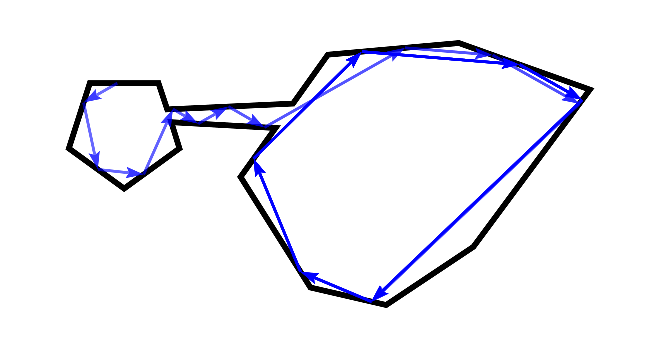
\includegraphics[width=\linewidth]{twoc_a_new.eps}
\end{subfigure}%
\begin{subfigure}{0.5\columnwidth}
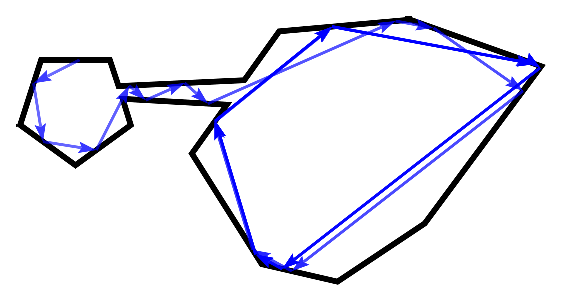
\includegraphics[width=\linewidth]{twoc_b.eps}
\end{subfigure}
\caption{Two paths produced by different sequences of bounces, which visit
different points of $\partial P$, yet have the same sequence of edge collisions 
and high-level dynamical behavior (escape the room on the left, travel through hallway, then
patrol the room on the right in a periodic orbit).\label{fig:twopaths}}
\end{figure}


\subsection{Purpose of this Document}

This document is meant to serve as documentation of the data structures we have
been developing to analyze bouncing robot systems, and a store for 
statements and proofs of mathematical properties thus far proven about the
systems.

The implications of our results for planning are broad, and depend on the
desired application of the robotic system. In our case, we focus our examples on
generating minimalist strategies such as constant bounce rules. We are
interested both in the theoretical questions of what tasks are possible with
such strategies, and in applications such as manufacture of micro-scale robots
that use mechanical interactions with boundaries to execute the bounce rules and
thus cannot be programmed with high-resolution strategies or complex on-board
state estimation.

This paper is intended to serve as a living document and additions, corrections, and
technical documentation of related softwares can be found online
\footnote{\url{https://github.com/alexandroid000/bounce_viz}}.

\section{Related Work}

We incorporate techniques from computational geometry, specifically visibility
\cite{ghosh2007visibility}. Visibility has been considered extensively in
robotics, but usually with the goal of avoiding obstacles
\cite{lozano1979algorithm,SimLauNis00}. To plan over collisions, we use the edge
visibility graph, analyzed in \cite{rourke_viz}, and shown to be strictly more
powerful than the vertex visibility graph. Our work is also related to problems
that consider what parts of a polygon will be illuminated by a light source
after multiple reflections (as if the edges of the polygon are mirrors)
\cite{Aronov1996}, or with diffuse reflections \cite{prasad1998visibility},
which are related to our nondeterministic bounces.

Our robot motion model is related to
\emph{dynamical billiards} \cite{billiards}. Modified billiard systems have attracted recent interest
\cite{DelMagno2014,pinball,billiards}. One similar work was inspired by the
dynamics of microorganisms; in \cite{microorganism2017}, the authors show that
\textit{Chlamydomonas reinhardtii} ``bounce'' off boundaries at a specific
angle determined by their body morphology. They characterize periodic and
chaotic trajectories of such agents in regular polygons, planar curves, and
other environments. Our model is especially interesting in this domain because
high-fidelity state estimation and control is often not possible at small
scales. It becomes necessary to make different assumptions about available
motion primitives, and our assumptions are more physically realistic as
micro-swimmers can often be constructed to have a default forward swimming
behavior and have predictable, mechanical interactions with boundaries
\cite{li2014hydrodynamic}.

Our motion model is a
form of \emph{compliant motion}, in which task constraints are used to guide task
completion, even when the exact system state is not known. Our use of
contraction mappings and nondeterministic reasoning is
related to the idea of \emph{funnels}: using
the attraction regions of a dynamical system to guide states into a goal region.
These ideas have been developed in the context of manipulation and fine motion control by Whitney
\cite{Whi77}, Mason \cite{Mas85}, Erdmann
\cite{Erd86}, Goldberg \cite{Gol93}, Lozano-P{\'e}rez, Mason, and Taylor
\cite{LozMasTay84}, Lynch and Mason \cite{LynMas95}, and Burridge, Rizzi, and Koditschek
\cite{BurRizKod99}, among many others. What we term {\em safe} planning is also
related to {\em conformant} planning \cite{anders2018reliably}, where given a set of possible initial configurations, a set of
nondeterministic actions, and a set of goal configurations, the planner should
find a sequence of actions guaranteed to bring the system into the goal. 


Our intentional use of collisions with
environment boundaries is enabled by the advent of more robust, lightweight mobile
robots. Collisions as information sources have also been
recently explored for multi-robot systems \cite{mayya2018localization}.
The first-class study of the dynamical properties of bouncing was proposed in
\cite{ErLav13} and continued in \cite{NilBecLav17}. Here we extend and improve
these analysis tools, and incorporate visibility properties to
discretize the strategy space. Work in contact planning for polygonal objects is
very closely related, and we use similar techniques for discretizing and
planning over the polygon boundary as seen in \cite{allen2015two}; this caging
problem is almost an ``external" version of our problem, albeit without the
aspect of long-term trajectory design.

In \cite{alam2017minimalist} and \cite{alam2018space}, the authors describe
navigation, coverage, and localization algorithms for a robot that rotates a fixed amount 
relative to the robot's prior heading. Due to the chosen state space discretization, 
periodic trajectories may exist which require bounce angles not allowed by the
discretization. By using a discretization induced by the environment geometry,
we are able to find all possible limit cycles, and the controllers necessary to
achieve them.
Another closely related work is \cite{LewOKa13}, which considered
navigation for a robot that has our same motion model, with uncertainty given as input to the
algorithm. This uncertainty bound is used to create a boundary discretization
using similar visibility properties as our approach, and the resulting
discretized space is searched for plans. In our case, instead of taking error bounds as input, our approach
considers all possible amounts of uncertainty, and returns bounds on the required
accuracy for strategies. This group has also recently extended their approach to
the coverage problem \cite{lewis2018guaranteed}.

We are working toward a generalization and hierarchy of robot models, in a
similar spirit to \cite{brunner2008simple}. Their {\em simple
combinatorial robot} is able to detect all visible vertices and any edges
between them, and move straight toward vertices. By augmenting this basic robot model
with sensors they construct a hierarchy of these robot models. Our questions are related but 
different: if the robot is given a compact, purely combinatorial environment representation, 
what tasks can it accomplish with minimal sensing, and how can we generate
minimal complexity, robust plans?



\section{Model and Definitions} \label{secmodel}

We consider the movement of a point robot in a simple polygonal environment,
potentially with polygonal obstacles. All index arithmetic for polygons with $n$ vertices is mod $n$ 
throughout this paper. We do not require polygons in general position. We do
not consider trajectories that intersect polygon vertices. We define our robot to move forward in a straight line, until
encountering an environment boundary (such as when a bump or range sensor is
triggered). Once at a boundary, the robot is able to rotate in place. More formally, the model is:
\begin{itemize}
\item The \emph{configuration space} $X = \partial P \times S^1$. $P$ is a simple polygon,
potentially with holes. $P$ has boundary $\partial P$, the union of external
and obstacle boundaries. $S^1$ is the robot's orientation in the plane. Let $s$ refer to a point in $\partial P$ without an associated robot orientation.
\item The \emph{action space} $U = [0,\pi]$, where $u \in U$ is the
orientation the robot takes when it reaches an environment boundary, before
moving forward again. $u$ is measured counterclockwise
relative to the boundary tangent. 
\item The \emph{state transition function} $f: X \times U \to X$, which
describes how actions change the state of the robot. We will often lift this function to act nondeterministically over sets
of states and actions, propagating each state forward under each possible action,
and unioning the resulting set of states. 
\item We model time as proceeding in stages; at each stage $k$, the robot
is in contact with the environment boundary, executes an action $u_k$, and then
moves forward until the next contact with the boundary at stage $k+1$.
\end{itemize}


\begin{definition}
Let $\alpha \in (0,\pi)$ be the robot's incoming heading relative to the
environment boundary at the point of contact. Let $\theta \in (0,\pi)$ be a control parameter. A 
\textbf{bounce rule} $b$ maps $\alpha$ and $\theta$ to an action
$u$, and determines how the robot will reorient itself when it collides with a
boundary. Bounce rules are defined in the
frame in which the environment normal is aligned with the positive $y$ axis and the
robot's point of contact with the boundary is the origin.
\end{definition}
\begin{definition}
A \textbf{nondeterministic bounce rule} is a bounce rule lifted to return a set of actions. 
We will restrict nondeterministic bounce rules to
return a convex set of actions (a single interval in $(0, \pi)$).
\end{definition}

For example, a specular bounce (laser beams, billiard balls) has bounce rule 
$b(\alpha, \theta) = \pi - \alpha$. See Figure \ref{fig:bex} for more
examples of bounce rules. 

\begin{figure}
    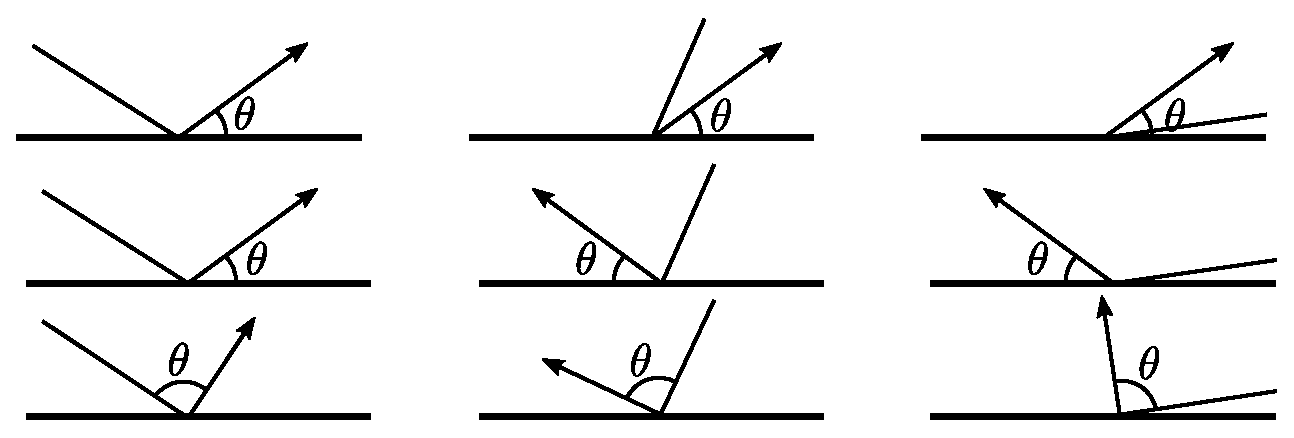
\includegraphics[width=0.9\columnwidth]{bounce_examples.eps}
    \centering
    \caption[test]{\label{fig:bex}Examples of different ``bounce rules'' that can be implemented on
mobile robots. In the first row, $b(\alpha, \theta) = \theta$, which we refer to
as a \textbf{fixed} bounce rule. In the second row, we have a \textbf{monotonic
fixed} bounce rule, in which
$b(\alpha, \theta) = \theta$ or $\pi-\theta$, depending on what is necessary to
preserve monotonicity of travel direction along the $x$ axis. In the third
row, we have a \textbf{relative} bounce rule, $b(\alpha, \theta) = \alpha - \theta$, rotating $\alpha$ through $\theta$ in the clockwise
direction. If this rotation causes the 
heading of the robot to still be facing into the boundary, the robot 
performs the rotation again until its heading points into the free space.
}
\end{figure}

\begin{definition}
A \textbf{bounce strategy} is a sequence of nondeterministic bounce rules.
\end{definition}

Of course, robots rarely move perfectly, so our analysis will assume the
robot has some nondeterminism in its motion execution.
Instead of modelling explicit
distributions, we assume the robot may execute any action in a set. 
Planning over such nondeterminism can result in design constraints
for robots; for example, if a robot has an uncertainty distribution over its 
actions in the range $u \pm \epsilon$, the largest allowable $\epsilon$ will 
be half the width of the smallest convex bounce rule interval in a strategy.

\section{Visibility-Based Boundary Partitioning} \label{secviz}

Given a polygonal environment (such as the floor plan of a warehouse or office
space), we would like to synthesize bounce strategies that allow a robot to
perform a given task (such as navigation or patrolling).
To do so, we first discretize the continuous space of all possible
transitions between points on $\partial P$. We find a visibility-based partition
that encodes the idea of some points on $\partial P$ having different
available transitions.

\begin{definition}
The \textbf{visibility polygon} of a point $s$ in a polygon $P$ is the polygon
formed by all the points in $P$ that can be connected to $s$ with a line
segment that lies entirely within $P$.
\end{definition}
%%S Are there any open/closed set issues with this?  Ambiguous?

Imagine a robot sliding along the boundary of a polygon, calculating 
the visibility polygon as it moves. In a convex polygon, nothing exciting 
happens. In a nonconvex polygon, the reflex vertices (vertices with an
internal angle greater than $\pi$) cause interesting
behavior.
As the robot slides, its visibility polygon mostly changes continuously. Edges
shrink or grow, but the combinatorial structure of the polygon remains the same,
until it aligns with a reflex vertex $r$ and another vertex $v$ (visible
from $r$). At this point, either 
$v$ will become visible to the robot, adding an edge to the visibility 
polygon, or $v$ will disappear behind $r$, removing an edge from the visibility polygon.


To compute all such points at which the visibility polygon changes structure, we
 compute the \textbf{partial local sequence}, defined in \cite{rourke_viz}.
These are, equivalently, the points where the combinatorial visibility vector
changes, as defined in \cite{suri2008simple}.
Each point in the partial local sequence marks the point
at which a visible vertex appears or disappears behind a reflex vertex. 
The sequence is constructed by shooting a ray through each reflex vertex $r$ from every
visible vertex and keeping the resulting sequence of intersections with
$\partial P$. See Figure \ref{fig:alg1} for an
example of the vertices in the partial local sequence of $v_0$. 

Once all the partial local sequences have been inserted into the original
polygon, the resulting segments have the property that 
any two points in the segment can see the same edge set of the
original polygon (though they may see different portions of those edges).
See Algorithm \ref{algo:insert} for a pseudocode
description of this partitioning process. Algorithm
\ref{algo:insert} applies to polygons with or without holes; holes 
require more bookkeeping to correctly find visible vertices and shoot
rays. See Figure \ref{fig:bvd_holes} for an example partition of a polygon with
 holes. Let $P'$ be the polygon $P$ after application of Algorithm
\ref{algo:insert}.

\begin{algorithm}
\caption{\textsc{PartitionPoly}(P)}
\label{algo:insert}
\hspace*{\algorithmicindent} \textbf{Input:} A polygon $P$ as a list of
vertices in counterclockwise order.\\
\hspace*{\algorithmicindent} \textbf{Output:} $P'$: $P$ with
all partial local sequence points added as new vertices.
\begin{algorithmic}[1]
\State $v_{new} \gets \{\}$
\State $reflex\_verts \gets$ \Call{GetReflexVerts}{$P$}
\For{$v_r$ in $reflex\_verts$}
    \For{$v_{vis}$ in \Call{VisibleVerts}{$P, v_r$}} 
        \State $v_{new} \gets$ $v_{new} \cup$ \Call{ShootRay}{$v_{vis}, v_r$}
    \EndFor
\EndFor
\State $P' \gets$ \Call{InsertVerts}{$v_{new}, P$}
\State \textbf{return} $P'$
\end{algorithmic}
\end{algorithm}

The $\textsc{ShootRay}$ function takes two visible vertices $v_{1}$ and $v_{2}$
and compute the first intersection of $\partial P$ and ray $v_{1}v_{2}$. This
operation will take $O(\log n)$ time after preprocessing the polygon $P$ in
$O(n)$ \cite{Szirmay-Kalos:1998:WVA:297217.297219}. The $\textsc{VisibleVerts}$
function computes all visible vertices in the polygon given an input query
vertex, and takes $O(n)$ \cite{ElGindy1981ALA}. So the total runtime of
Algorithm 1 is $O(n^2\log n)$.

\begin{definition}
The \textbf{edge visibility graph} of a polygon $P$ has a node for each edge of
$P$, and has an arc between two nodes $(e_i, e_j)$ if and only if there is a
point $s_i$ in the open edge $e_i$ and a point $s_j$ on the open edge $e_j$ such
that $s_i$ and $s_j$ can be connected with a line segment which is entirely
within the interior of $P$.
\end{definition}


\begin{figure}[h]
\centering
\begin{subfigure}{0.5\columnwidth}
    \centering
    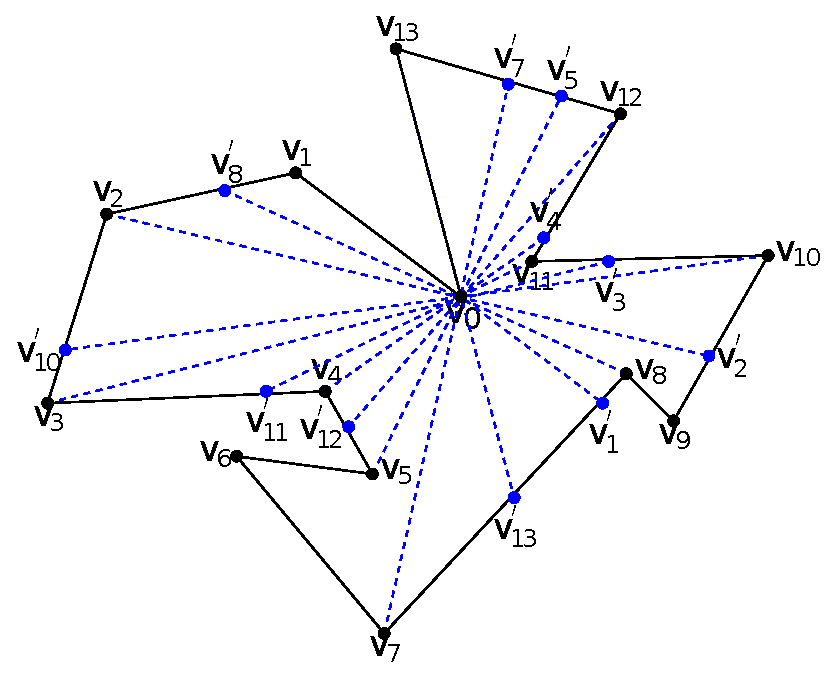
\includegraphics[width=\linewidth]{tikz1.eps}
\end{subfigure}%
\begin{subfigure}{0.5\columnwidth}
    \centering
    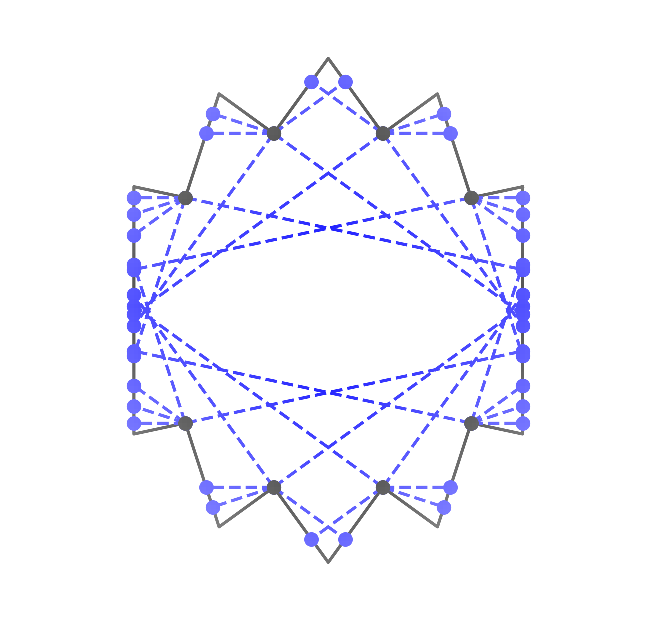
\includegraphics[width=\linewidth]{chestnut_5.eps}
\end{subfigure}
\centering
\caption{On the left, the partial local sequence for $v_0$. On the right, an example polygon for which the bounce visibility graph has
$O(n^4)$ edges.\label{fig:alg1}}
\end{figure}

Let the \textbf{bounce visibility graph} be the directed edge visibility graph of
$P'$. Although visibility is a symmetric property, we use directed edges in the
bounce visibility graph so that 
we can model the 
geometric constraints on the visibility from one edge to another, which are
not symmetric and govern what actions allow the robot to accomplish that
transition. See Section \ref{sec:safe} for further exploration of this idea.



\begin{proposition} \label{prop:complexity}
The bounce visibility graph for a polygon with $n$ vertices has 
$O(n^2)$ vertices and $O(n^4)$ edges.
\end{proposition}

\begin{proof}

Consider a polygon $P$ with $n$ vertices operated on by Algorithm
\ref{algo:insert} to form $P'$. Each convex vertex will not add any new vertices; however, 
a reflex vertex can add $O(n)$ new vertices. Up to half of the vertices in the polygon 
can be reflex, so the number of vertices in $P'$ is $O(n^2)$. 
Each vertex indexes a node in the edge visibility graph of $P'$. A vertex 
in $P'$ may be visible to all other vertices, so in the worst
case, the bounce visibility graph will have $O(n^4)$ edges. \qed

\end{proof}

\subsubsection*{Worst Case Example for Algorithm \ref{algo:insert}}

We might hope that if $r$ is large, then not all of the reflex vertices will
produce a large number of new vertices, and we may bound the size of the edge
set in the visibility graph. Unfortunately, the number of reflex
vertices, the new vertices produced in their partial local sequence, and the new
vertices' visibility can be large at the same time. We will present a family of
input polygons with bounce visibility graph edge-set size of $O(n^4)$.

Let $n = 4t+2$, in which $t$ is a positive integer. We design a polygon with
$r = 2t$ reflex vertices. The polygon is symmetric with respect to its medium
horizontal line. In the top half, the reflex vertices are uniformly located on a
circle and thus they are visible to each other; the convex vertices are chosen
so that they are outside the circle and the line through an edge will not
intersect other edges. Each reflex vertex will have at least $t-1$ new
vertices in its partial local sequence. There will be $2t(t-1)+n$
vertices in the polygon after we insert all new vertices in the partial local
sequence for all reflex vertices. Each of them can see at least $t(t-1)+n/2$
other vertices. Thus the number of edges in the transition graph for the
polygon with inserted vertices is
$O ((2t(t-1)+n)(t(t-1)+n/2)) = O(t^4) = O(n^4)$.
Fig \ref{fig:alg1} shows the polygon for $t = 4$ with all the
vertices in the partial local sequences.

\begin{figure}
\begin{subfigure}{0.5\columnwidth}
\centering
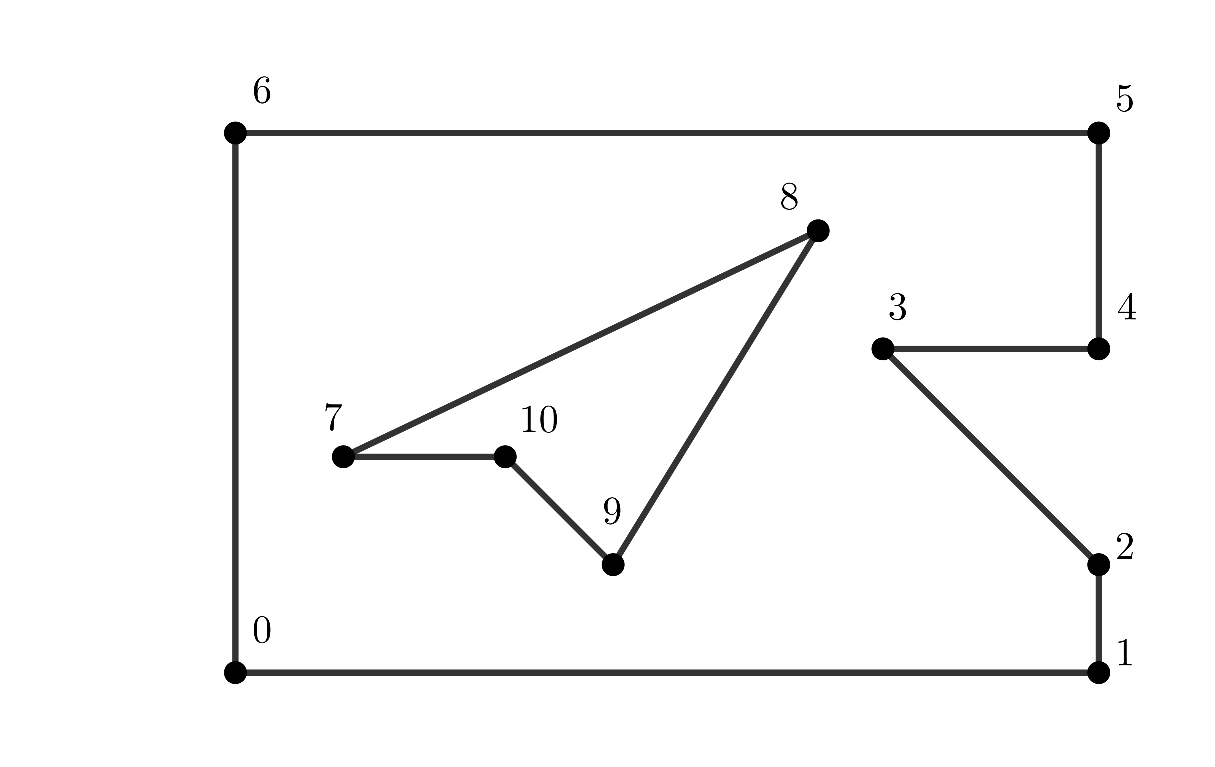
\includegraphics[width=0.9\linewidth]{median_holes.eps}
\centering
\end{subfigure}%
\begin{subfigure}{0.5\columnwidth}
\centering
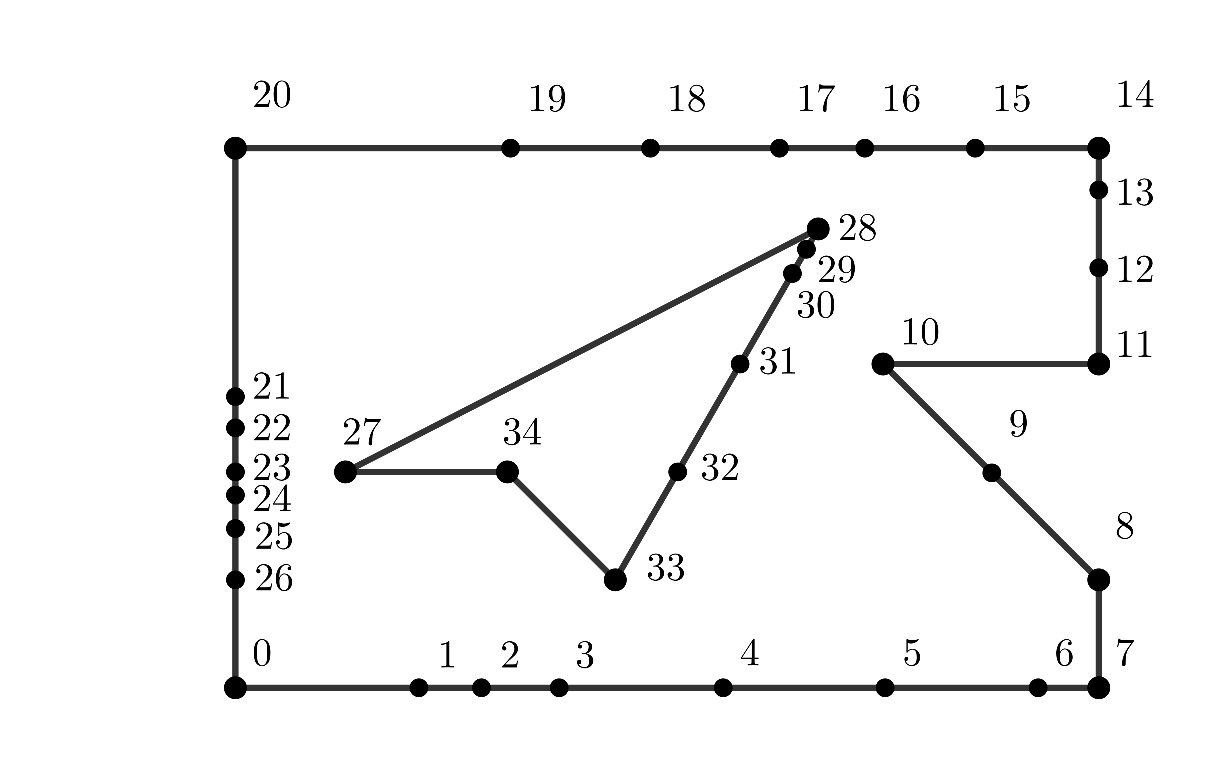
\includegraphics[width=0.9\linewidth]{median_holes_inserted.eps}
\centering
\end{subfigure}
\caption{An example partition for a polygon with holes; our discretization
scheme extends naturally to handle visibility events caused by static obstacles.}
\label{fig:bvd_holes}
\end{figure}

\section{Safe Actions} \label{sec:safe}

To characterize some families of paths, we will use the boundary
partition technique defined in Section \ref{secviz}, then define
\emph{safe actions} between segments in the partition that are
guaranteed to transition to the same edge from anywhere in the
originating edge. Such actions define transitions which keep the
robot state in one partition under nondeterministic actions.

\begin{definition}
Two edges $e_i,e_j$ of a polygon are \textbf{entirely visible} to each other if
and only if every pair of points $s_i \in e_i$ and $s_j \in e_j$ are visible (the
shortest path between $s_i$ and $s_j$ lies entirely within $P$).
\end{definition}

\begin{definition} \label{def:sa}
A \textbf{safe action} from edge $e_i$ to edge $e_j$ in a polygon is an 
action $u$ such
that $f(s,u) \in e_j$ for any $s \in e_i$ and $u$ in some interval of actions
$\tilde{\theta} \subseteq (0,\pi)$.
\end{definition}

\begin{proposition} \label{prop:saferange}
Given two entirely visible line segments $e_i = (v_i, v_{i+1})$ and $e_j =
(v_j, v_{j+1})$ in $\partial P'$, if a safe action
exists from $e_i$ to $e_j$, the maximum interval of safe actions is $\bm{\tilde{\theta} = [\theta_r, \theta_l]}$ such
that $\theta_r = \pi - \angle v_j v_{i+1} v_i$ and $\theta_l = \angle v_{j+1}
v_i v_{i+1}$.
\end{proposition}

\begin{proof}

Let edge $e_i = (v_i, v_{i+1})$ be aligned with the positive $x$ axis with the clockwise
endpoint at the origin, without loss of generality. 
Due to the edges being
entirely visible, $e_j = (v_j, v_{j+1})$ must be in the top half of the plane, above
$e_i$.

Take the quadrilateral formed by the convex hull of the edge endpoints.
Let the edges between $e_i$ and $e_j$ be $e_l = (v_i, v_{j+1})$ and the right-hand edge 
$e_r = (v_{i+1}, v_j)$. Let $\theta_{l}$ be
the angle between $e_l$ and the positive $x$ axis ($0 < \theta_l < \pi$); similarly
for $e_r$ and $\theta_r$. See Figure \ref{fig:bounce_range} for an illustration of
the setup. 

\begin{figure}
    \centering
    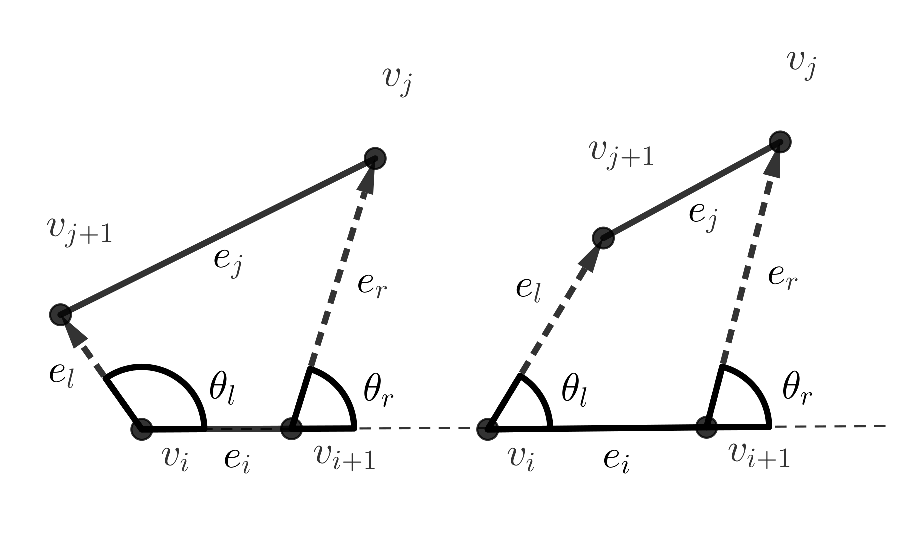
\includegraphics[width=0.8\columnwidth]{bouncerange_min.eps}
    \caption{Angle range such that a transition exists for all points on
originating edge (left: such a range exists, right: such a range does not
exist)}
\label{fig:bounce_range}
\end{figure}


There are three cases to consider: if $e_l$ and $e_r$ are extended to infinity,
they cross either above or below edge $e_i$, or they are parallel.

\emph{Case 1:} $e_l$ and $e_r$ meet below edge $e_i$. In this case,
$\theta_l > \theta_r$ and if a ray is cast from any point on $e_i$ at angle
$\theta \in [\theta_r, \theta_l]$, the ray is guaranteed to intersect $e_j$ in its
interior.

\emph{Case 2:} $e_l$ and $e_r$ meet above edge $e_i$. In this case, $\theta_l <
\theta_r$, and there is no angle
$\theta$ such that a ray shot from \emph{any} point on $e_i$ will intersect
$e_j$.
To see this, imagine sliding a ray at angle $\theta_l$ across the quadrilateral
- at some point before reaching $v_{i+1}$, the ray must stop intersecting $e_j$,
else we would have $\theta_l > \theta_r$.

\emph{Case 3:} $e_l$ and $e_r$ are parallel. This implies that $\theta_{l} =
\theta_{r}$, which is the only angle for which a transition from any
point on $e_i$ is guaranteed to intersect $e_j$, and $\tilde{\theta}$ is a
singleton set.

Thus, for each case, we can either compute the maximum angle range or determine
that no such angle range exists. \qed

\end{proof}

Note that this definition of a safe action is similar to the definition of an interval of
safe actions from \cite{LewOKa13}; the main differences in approach are the
generation of boundary segments, methods of searching the resulting graph, and
how we generate constraints on robot uncertainty instead of assuming uncertainty
bounds are an input to the algorithm.

\begin{lemma} \label{lem:action}
If two edges in $\partial P'$ are entirely visible to each other, then there will be at least one safe
action between them.
\end{lemma}

\begin{proof}
From the proof of Proposition \ref{prop:saferange}, we can see that if case one
holds in one direction, case two will hold in the other direction, so a safe
action must exist from one edge to the other in one direction. If case three
holds, there is a safe action both directions but $\tilde{\theta}$ is a
singleton set. \qed
\end{proof}


\begin{corollary} \label{coro:neighbor}
If two edges in $\partial P'$ share a vertex that is not reflex, and the two
 edges are not collinear, then there exist safe actions
from one to the other in both directions.
\end{corollary}

For a proof of Corollary \ref{coro:neighbor}, see Figure \ref{fig:safe_action_1}.
Algorithm \ref{algo:insert} guarantees that such neighboring segments are
entirely visible.

\begin{definition}
Given two entirely visible segments $e_i$ and $e_j$,
rotate frame such that $e_i$ is aligned with the $x-$axis with its normal pointing
along the positive $y-$axis, such that 
segment $e_j$ is above segment $e_i$. If the intersection of segment $e_i$ and
$e_j$ would be on the left of segment $e_i$, then call the transition from $e_i$ to $e_j$ a
\textbf{left
transition}; if the intersection would be on the right of segment $e_i$, then call the
transition a \textbf{right transition}.
\end{definition}

\begin{proposition} \label{prop:twosafe}
For every polygon $P$ and the resulting partitioned polygon $P'$ under Algorithm
\ref{algo:insert}, each edge $e \in P'$ has at least two safe actions which allow
transitions away from $e$.
\end{proposition}

\begin{proof}

Let $e_i = (v_i, v_{i+1})$. Consider right transitions from $e_i$ to some $e_k$,
where the safe action interval $\tilde{\theta} = (0, \theta_l)$ for some 
nonzero $\theta_l$. We will show that such a transition must exist. 

By Corollary \ref{coro:neighbor}, if an edge $e_i$ has an adjacent edge
$e_{i+1}$ which is not collinear or separated by a reflex angle, 
$e_k = e_{i+1}$ and a safe transition exists
between $e_i$ and $e_{i+1}$ with $\theta_l = \angle v_{i+2} v_i v_{i+1}$. 
See Figure \ref{fig:safe_action_1}.

If the adjacent edge is at a reflex angle, Algorithm 
\ref{algo:insert} will insert a vertex in line with $e_i$ on the closest visible
edge, forming edge $e_k$. If $v_i$ is an original
vertex of $P$, $e_k$ will be entirely visible from $e_i$, since Algorithm
\ref{algo:insert} will otherwise insert a point in $v_i$'s partial local
sequence.

If $v_i$ is itself inserted by Algorithm \ref{algo:insert}, $e_k$ will still be
entirely visible. There must be some original vertex of $P$
clockwise from $v_i$ and collinear with $e_i$, which would insert a vertex
visible to $e_i$ through Algorithm \ref{algo:insert} if there were any reflex vertices
blocking transitions to $e_k$.
See Figure \ref{fig:safe_action_3} for an example of the geometry.

If the adjacent edge $e_{i+1}$ is collinear with $e_i$, apply the above reasoning 
to the first non-collinear edge to find $e_k$.
The above arguments extend symmetrically to left transitions, which will have
safe actions of the form $\tilde{\theta} = [\theta_r, \pi)$. Thus, each edge will 
have two guaranteed safe actions leading away from it. \qed
\end{proof}

\begin{figure}
\centering
\begin{subfigure}{0.5\columnwidth}
\centering
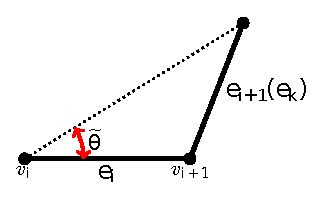
\includegraphics[width=0.9\columnwidth]{tikz2.eps}
\captionof{figure}{\label{fig:safe_action_1}}
\end{subfigure}%
\begin{subfigure}{0.5\columnwidth}
\centering
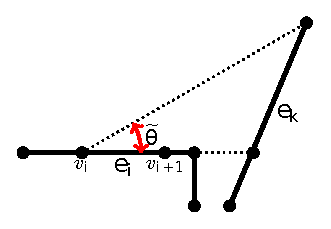
\includegraphics[width=0.9\columnwidth]{tikz3.eps}
\captionof{figure}{\label{fig:safe_action_3}}
\end{subfigure}
\caption{Examples of geometrical setup for some guaranteed safe actions.}
\label{fig:two_safe_cases}
\end{figure}


\section{Dynamical Properties of Paths} \label{secdyn}


Many robot tasks can be specified in terms of dynamical properties of
the path the robot takes through space: stability, ergodicity, etc.
Our motion strategy allows us to disregard the robot's motion in the interior of
$P$. Instead, the robot's state is an interval 
along the boundary $\partial P$, and we can formulate transitions as a discrete
dynamical system under the transition function $f$. The properties of this
dynamical system can be used to engineer paths corresponding to different robot
task requirements.

One generally useful property of mapping functions is \emph{contraction}: 
when two points under the function always become closer together. 
We can use this property to control uncertainty in the robot's position.

\begin{definition}
Let $\bm{\phi_{i,j}}$ be the interior angle between two edges $e_i, e_j \in \partial P$. 
\end{definition}

\begin{definition}

A function $g$ that maps a metric space $M$ to itself is a \textbf{contraction
mapping} if for all
$x, y \in M$, $\lvert g(x) - g(y) \rvert \leq c \lvert x-y \rvert$, and $0 \leq c < 1$.
\end{definition}

\begin{lemma} \label{lemma:angrange}
If the transition from segment $e_i$ to segment $e_j$ is a left transition, then the
transition function $f(x, \theta)$ between segments $e_i$ and $e_j$ is a contraction
mapping if and only if $\theta > \frac{\pi}{2}+\frac{\phi_{i, j}}{2}$;
if a right transition, the transition function $f(x, \theta)$ is a contraction mapping if
and only if $\theta < \frac{\pi}{2}-\frac{\phi_{i, j}}{2}$.
\end{lemma}

\begin{proof}

\begin{figure}
    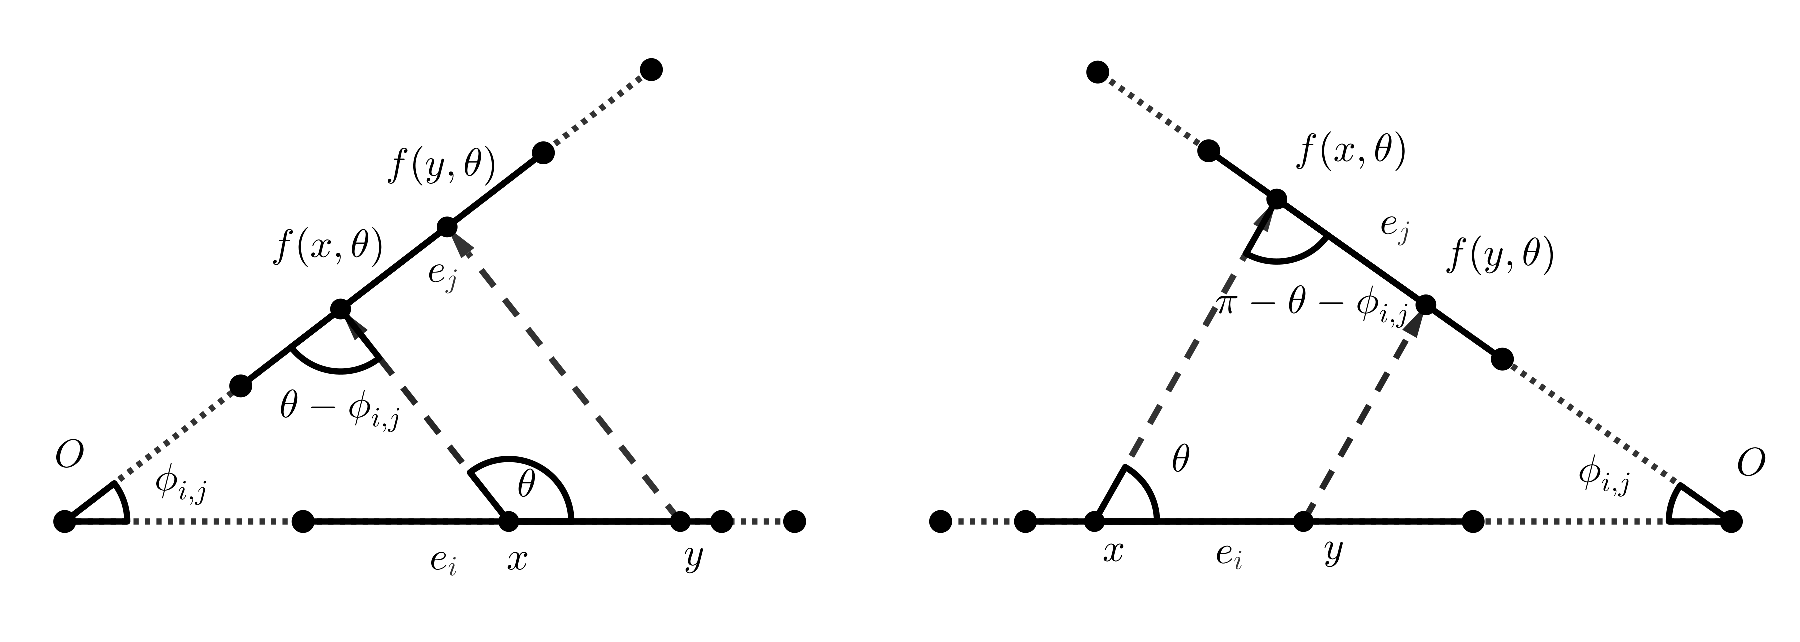
\includegraphics[width=0.9\columnwidth]{contraction_map_cond.eps}
    \centering
    \caption{The two cases for computing contraction mapping conditions. \label{fig:cont_map}}
    \centering
\end{figure}

We consider the two cases of transition separately:
\begin{enumerate}
    \item For the transition shown in the left hand side of Figure~\ref{fig:cont_map}, 
          $\overline{xf(x, \theta)} \parallel \overline{yf(y, \theta)} \Rightarrow \frac{|f(x, \theta)-f(y, \theta)|}{|x-y|} = \frac{|f(x, \theta)|}{|x|} = \frac{\sin(\pi - \theta)}{\sin(\theta - \phi_{i, j})} = \frac{\sin(\theta)}{\sin(\theta-\phi_{i, j})}.$ The transition will be contraction if and only if $\frac{|f(x, \theta)-f(y, \theta)|}{|x-y|} < 1 \iff \sin(\theta)<\sin(\theta-\phi_{i, j})$. If $\theta < \frac{\pi}{2}$, then $\sin(\theta) > \sin(\theta-\phi_{i, j})$. Thus we need $\theta>\frac{\pi}{2}$. If $\theta-\phi_{i, j} > \frac{\pi}{2}$, then $\sin(\theta) < \sin(\theta-\phi_{i, j})$ and we are done; otherwise we need $\pi - \theta < \theta-\phi_{i, j} \Rightarrow \theta - \frac{\phi_{i, j}}{2} > \frac{\pi}{2}$. Combining all conditions, we have the transition will be contraction if and only if $\theta >\frac{\pi}{2} + \frac{\phi_{i, j}}{2}$.
    \item Similarly, for a right transition shown in the right diagram of
Figure \ref{fig:cont_map},
$\overline{xf(x, \theta)} \parallel \overline{yf(y, \theta)} \Rightarrow \frac{|f(x, \theta)-f(y, \theta)|}{|x-y|} = \frac{|f(x, \theta)|}{|x|} = \frac{\sin(\pi - \theta)}{\sin(\pi -\theta-\phi_{i, j})} = \frac{\sin(\theta)}{\sin(\theta + \phi_{i, j})}.$
The transition will be contraction if and only if
$\frac{|f(x, \theta)-f(y, \theta)|}{|x-y|} < 1 \iff \sin(\theta)<\sin(\theta+\phi_{i, j})$.
If $\theta > \frac{\pi}{2}$, then $\sin(\theta) > \sin(\theta + \phi_{i, j})$.
Thus we need $\theta<\frac{\pi}{2}$. If $\theta+\phi_{i, j} < \frac{\pi}{2}$,
then $\sin(\theta) < \sin(\theta+\phi_{i, j})$ and we are done; otherwise we
need
$\theta < \pi-\theta-\phi_{i, j} \Rightarrow \theta < \frac{\pi}{2} - \frac{\phi_{i, j}}{2}$.
Combining all conditions, we have the transition will be contraction if and only
if $\theta <\frac{\pi}{2} - \frac{\phi_{i, j}}{2}$. \qed
\end{enumerate}
\end{proof}

%In our case, we will always take $M$ to be an interval in $\mathbb{R}$ and we
%will use the L1 norm. The proof is a straightforward application of the law of
%sines to find the conditions for the contraction coefficient $\frac{ | f(x,\theta)-f(y,\theta)
%|}{|x-y|}$ to be less than one, which is independent of choice of interval $[x, y]$ for transitions between linear
%segments, and is very similar to the calculations in \cite{NilBecLav17}.

\begin{corollary} \label{coro:existcontract}
For all pairs of adjacent 
segments with internal angle less than $\pi$,
there exists a range of actions for which $f$ is a contraction mapping.
\end{corollary}

\begin{definition} \label{def:cc}
The \textbf{contraction coefficient} of a mapping is the ratio of the distance between points before and after
the mapping is applied.
Let $C(\theta, \phi_{i, j})$ be the contraction coefficient of a transition from $e_i$ to $e_j$ in $\partial P$
For a left transition, $C(\theta, \phi_{i, j}) = | \frac{\sin(\theta)}{\sin(\theta - \phi_{i, j})} |$; 
for a right transition,  $C(\theta, \phi_{i, j}) = | \frac{\sin(\theta)}{\sin(\theta + \phi_{i, j})} |$.
\end{definition}

Given $C$ from Definition \ref{def:cc}, for a sequence of transitions $f_0, \ldots, f_k$, 
we can construct the overall mapping from the domain of $f_0$ to the range of $f_k$ through function
composition. Since $f$ is a linear mapping, the contraction coefficient of a composition 
of multiple bounces can be determined by multiplying the contraction
coefficients of each bounce.

\begin{definition} \label{def:c}
Given a sequence of $m$ feasible transitions $F = \{f_0, f_1, \ldots, f_{m-1}\}$, at stage $k$ the robot 
will be located on edge $e(k)$ and will depart the edge with
action $\theta_k$; the contraction coefficient of the overall robot
trajectory $f_{m-1} \circ \ldots \circ f_0$ is $C(F) = \prod_{k=0}^{m-1} C(\theta_{k}, \phi_{e(k), e(k+1)})$.
\end{definition}

If $C(F) < 1$, the composition of $F$ is a contraction mapping. This is true even if some transition along
the way is not a
contraction mapping, since $C(F)$ is simply the ratio of distances
between points before and after the mapping is applied. Furthermore, the value
of $C(F)$ tells us the exact ratio by which the
size of the set of possible robot states has changed.

\subsection{Limit Cycles} \label{sec:limcycles}
A contraction mapping that takes an interval back
to itself has a unique fixed point, by the Banach fixed point
theorem \cite{Granas2003}. By composing individual transition functions, 
we can create a self-mapping 
by finding transitions which take the robot back to its originating edge. A fixed
point of this mapping corresponds to a stable limit cycle.
Such trajectories in regular polygons were characterized in \cite{NilBecLav17}.
Here, we present a more general proof for the existence of limit cycles in all
convex polygons.

\begin{definition}
$\phi_{P,min}$ is the smallest interior angle in a polygon $P$.
\end{definition}

\begin{lemma} \label{lem:convex}
Consider $\theta \in (0,\frac{\pi}{2}]$, if 
\begin{equation*}
\theta \in (0, \min(\min_{i = 0, 1, \dots, n-1}(\angle v_{i+2}v_{i}v_{i+1}),
\min_{i = 0, 1, \dots, n-1}(\frac{\pi}{2}-\frac{\phi_{i-1, i}}{2}))),
\end{equation*}
then the fixed bounce rule $b(\alpha, \theta) = \theta$ leads to a convex cycle that visits each edge of $P$ sequentially, regardless of the robot's position.
For all convex polygons with $n$ edges, there exist constant fixed-angle bouncing
strategies which result in a period $n$ limit cycle regardless of the robot's start position.
\end{lemma}
\begin{proof}
\begin{figure}
    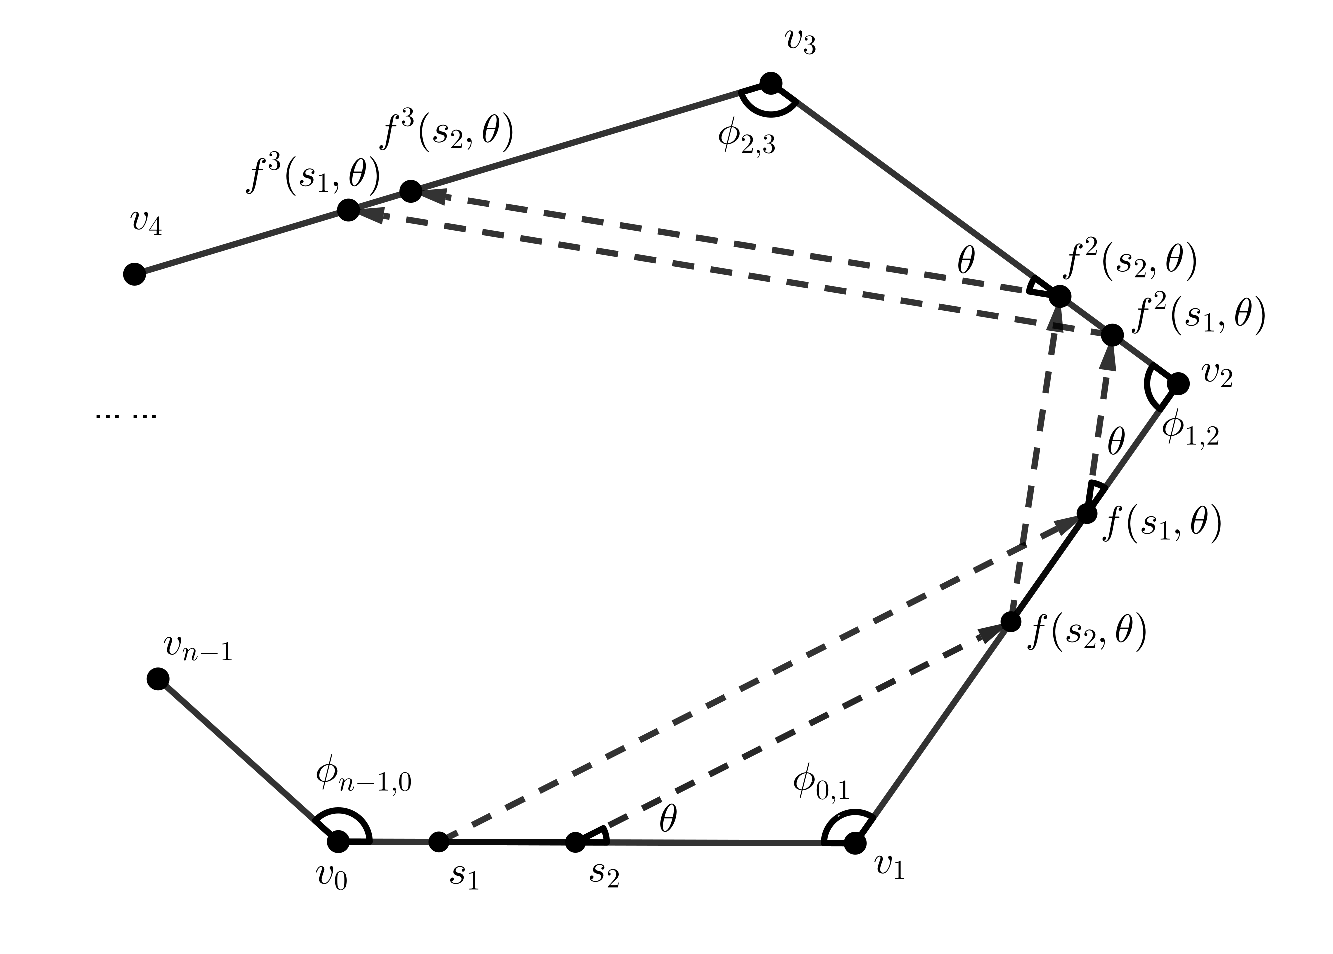
\includegraphics[width=0.9\columnwidth]{convex_cycle.eps}
    \centering
    \caption{The notation setup for the proof of contracting cycle in a convex polygon.\label{fig:conv_cycle}}
    \centering
\end{figure}

See Figure \ref{fig:conv_cycle} for the geometric setup.

Without loss of generality, assume $\theta \in (0, \frac{\pi}{2}]$. The robot will always bounce
to the next adjacent edge if and only if
$\theta \in (0, \min_{i}(\angle v_{i+2}v_{i}v_{i+1}))$.

Suppose we have two start positions $s_1$ and $s_2$ on edge $e_0$ and a constant fixed bounce 
rule $b(\alpha, \theta) = \theta$.
At stage $k$, $s_1$ and $s_2$ will be located at $f^{k}(s_1,\theta)$ and
$f^{k}(s_2,\theta)$. 

By Definition \ref{def:c}, the distance between $s_1$ and $s_2$ changes after one orbit of the polygon by the
ratio $\frac{\lvert f^{n}(s_1, \theta) - f^{n}(s_2, \theta) \rvert}{ \lvert s_1
- s_2 \rvert } = \prod_{i = 0}^{n-1}
C(\theta, \phi_{i, i+1})$. If this ratio is less than one, then $f^n(s,\theta)$ has a unique fixed point by the Banach fixed-point theorem
\cite{Granas2003}. By Lemma \ref{lemma:angrange}, this constraint is satisfied if  
$\theta < \frac{\pi}{2}-\frac{\phi_{i, i+1}}{2}$ for all $i$. We can guarantee that this
condition holds for the orbit by requiring

\begin{equation*}
\theta \in (0, \min(\min_{i = 0, 1, \dots, n-1}(\angle v_{i+2}v_{i}v_{i+1}),
\min_{i = 0, 1, \dots, n-1}(\frac{\pi}{2}-\frac{\phi_{i-1, i}}{2}))),
\end{equation*}

\noindent
in which case the fixed-angle bouncing strategy with $b(\alpha, \theta) = \theta$ leads to a convex
cycle which visits each edge of $P$ sequentially, regardless of the robot's start position.
Symmetry applies for orbits in the opposite direction. \qed
\end{proof}

So now we know that such cycles must exist in convex polygons, and we know the 
conditions on fixed bounce laws that will create them, but we can also compute
exactly {\em where} these cycles would be located (in the asymptotic limit).

For ease of notation, Theorem \ref{theo:fixedPoint} will compute the location of
counterclockwise limit cycle trajectories as a fixed point of the return map of the trajectory
starting on edge $e_0$. The rest of the points of the limit cycle can
be computed from forward projection of the trajectory, or from reindexing the
vertices and computing this distance for each edge. Clockwise limit cycles can
be computed through symmetry (flipping the polygon in the plane and computing
the cycle, then flipping back).

\begin{theorem}
\label{theo:fixedPoint}
Under a fixed bounce rule $b(\alpha, \theta) = \theta$ in a convex polygon with $n$ edges, 
if $\theta$ satisfies the conditions in Lemma~\ref{lem:convex} such that the trajectory will converge asymptotically to a limit cycle striking each sequential edge of the polygon in counter-clockwise order, then on edge $e_0$ the limit cycle will be located distance
\begin{equation}
\label{eq:fixedPoint}
d_{FP} =\frac{\sum_{j=0}^{n-1} (-1)^{n-j-1} \ell_j \prod_{k=j}^{n-1} C(\theta, \phi_{k, k+1})}
{1 - (-1)^n \prod_{k=0}^{n-1} C(\theta, \phi_{k, k+1})},
\end{equation}
from vertex $v_0$. 
\end{theorem}
\begin{proof}
Define a distance function, $d$, which measures the robot's linear distance
along the polygon boundary from the nearest clockwise vertex. If the robot bounces 
at angle $\theta$ between edges $e_i$ and $e_{i+1}$, the new distance $d(f(x, \theta))$ can be derived with the law of sines as
\begin{equation} \label{eq:dist}
d(f(x, \theta)) = \frac{\sin(\theta)}{\sin(\theta + \phi)} (\ell_0 - d(x)) =
C(\theta, \phi_{0,1}) (\ell_0 - d(x)).
\end{equation}

Now we define the return map, $f_{r}$, corresponding to bouncing $n$
times around an $n$-sided polygon until the robot returns to the originating
edge. The new distance of the returning robot from $v_0$ can be computed by
composing the distance functions of each transition, of the form in Equation~(\ref{eq:dist}). This return map will take the form
\begin{equation*}
\begin{aligned}
d(f_{r}(x, \theta)) ={} & C(\theta, \phi_{n-1, 0}) (\ell_{n-1}  - (C(\theta, \phi_{n-2, n-1})(\ell_{n-2} - \ldots \\
& - C(\theta, \phi_{0,1})(\ell_0 - d(x)) \ldots ))),
\end{aligned}
\end{equation*}
which can be expanded and grouped into

\begin{equation*}
\begin{aligned}
d(f_{r}(x, \theta)) ={} & 
\sum_{j=0}^{n-1} (-1)^{n-j-1} \ell_j \prod_{k=j}^{n-1} C(\theta, \phi_{k, k+1}) \\
& + d(x) (-1)^n \prod_{k=0}^{n-1} C(\theta, \phi_{k, k+1}).
\end{aligned}
\end{equation*}

And to find the fixed point of this return map (corresponding to the stable
limit cycle of the robot around the polygon), we set $d(f_{r}(x, \theta)) =
d(x)$, and solve for $d(x)$, yielding
$$
d(x) =\frac{\sum_{j=0}^{n-1} (-1)^{n-j-1} \ell_j \prod_{k=j}^{n-1} C(\theta, \phi_{k, k+1})}
{1 - (-1)^n \prod_{k=0}^{n-1} C(\theta, \phi_{k, k+1})},
$$
which in turn yields the expression for the the distance $d_{FP}$ from vertex $v_0$ that defines the fixed point. 
\end{proof}

While Equation~(\ref{eq:fixedPoint}) might look cumbersome, it is easy to compute (linear in the number of sides of the polygon). See Figure \ref{fig:fp} for an example of the predicted locations of the limit cycle in a convex polygon. The trajectory begins on the left hand side of the polygon and quickly converges to the predicted limit cycle.

\begin{figure}
\centering
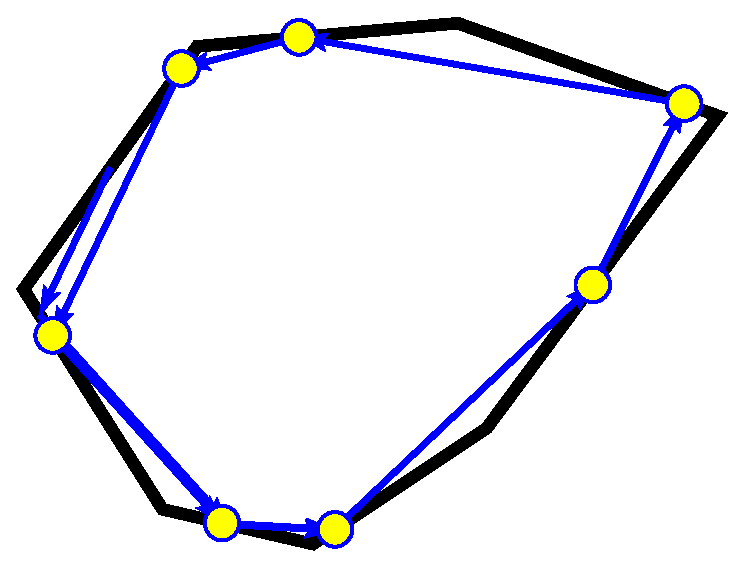
\includegraphics[width=0.8\columnwidth]{fixed_points_prediction.eps}
\caption{The blue arrows indicate an example
trajectory for a constant fixed bounce rule. Yellow circles indicate the 
predicted collision points of the
asymptotically stable limit cycle for this bounce rule and polygon.}
\label{fig:fp}
\end{figure}


\begin{proposition} \label{prop:cycle}
For all points $s$ on the boundary of all polygons, a constant
fixed-angle controller exists which will cause the robot's trajectory to enter a
stable limit cycle.
\end{proposition}

\begin{proof}
First we observe that by Proposition \ref{prop:twosafe}, for every segment $e
\in \partial P'$, 
safe actions always exist
for two action intervals. These intervals are the ones bordering the segment itself:
by staying close enough to the boundary, the robot may guarantee a safe
transition. By Lemma \ref{lemma:angrange}, these safe actions will also
admit contraction mappings. Thus, we may choose a constant fixed-angle
controller such that it results in safe, contracting transitions from all
segments in $P'$. Since there are a finite number of segments in $P'$, this
controller must result in limit cycle from every point in $P$. If $s$ is on a
hole of the polygon, this procedure will cause the robot to leave the hole and
enter a cycle on the exterior boundary. \qed
\end{proof}

\subsection{Leveraging Cycles to Reduce Uncertainty}

Next, we will detail how such cycles can be used to decrease uncertainty in the
robot's position.

\begin{corollary} \label{coro:shrink}
Choose a sequence of transitions $F$ that begins and ends on edge $e_i$. Let the
contraction coefficient of this trajectory be $C$, and let the length of edge $e_i$
be $\ell_i$. After $k$ iterations of the cycle,
the distance between the robot's position and the fixed point of the cycle's transition
function must be less than $C^k \ell_i$.
\end{corollary}

\begin{proof}
The initial distance between the robot's position and the fixed point of
the cycle, $|x_0 - x_{FP}|$, is upper bounded by $\ell_i$. After $F$ has been
executed once, the contraction ratio $C = \frac{|F(x_0) - F(x_{FP})|}{|x_0 -
x_{FP}|} = \frac{|F(x_0) - x_{FP}|}{|x_0 - x_{FP}|}$, which implies $|F(x_0) - x_{FP}|
= C |x_0 - x_{FP}| \leq C \ell_i$. When $F$ is iterated $k$ times, this
expression becomes $|F^k(x_0) - x_{FP}| \leq C^k \ell_i$. \qed
\end{proof}

\begin{corollary}

If we assume the robot's initial location lies in an interval on edge $e_i$, 
and the robot performs a sequence of transitions $F$ that creates a cycle
returning to $e_i$ with contraction coefficient $C$, the size of the set of
possible locations of the robot on edge $e_i$ will become less than $\epsilon$
after $\lceil \log(\epsilon/2 \ell_i)/\log(C) \rceil$ iterations of the 
cycle.
\end{corollary}

\begin{proof}

From Corollary \ref{coro:shrink}, after $k$ cycles the distance between the
robot's position and the fixed point will be less than $C^k \ell_i$. Thus, if we
wish for the size of the interval of possible positions to be less than
$\epsilon$, we must have that $C^k \ell_i = \epsilon / 2$. Solving for $k$
yields the expression above. \qed

\end{proof}


\section{Applications}

\subsection{Planning}

Here, we define the planning task, assuming that
the robot has unavoidable uncertainty in its actuation. We make no assumptions
on the distribution or size of uncertainty, only that it is bounded, so we can
plan over ``cones" (intervals of possible actions, which cause the robot's state
uncertainty to spread linearly as it moves through the interior).
A resulting strategy is should take a robot
from any point in a starting set to some point in a goal set, as long as some
action in the bounce rule set is successfully executed at each stage. 

First we will address the problem of safe planning using only geometric information, 
without incorporating the dynamical properties of the system, and show the limitations
of this approach. Then, we will show several methods and heuristics for
improving this situation using the dynamical properties described in Section
\ref{secdyn}.

\begin{definition}
\textbf{Safe Planning Problem}:
Given a polygonal environment $P$, a convex starting set $S \subset \partial P$ of possible robot positions along the
environment boundary, and a convex goal set $G \subset \partial P$, determine a strategy $\pi$ which
will be guaranteed to take the robot from any point in $S$ to a point in $G$, or
determine that no such strategy exists.
\end{definition}

Using the formalisms built up so far, we can tackle this problem by searching over
the bounce visibility graph, using it as a roadmap. Shortest paths in the graph 
will correspond to paths with the fewest number of bounces. It is important to
note that an arc $e_i \to e_k$ in the bounce visibility graph only implies that for each
point $x \in e_i$ there exists an action taking $x$ to some point in $e_k$. For
our task, we require a {\em range} of angles which can take {\em any}
point in $e_i$ to a point on $e_k$, so we restrict the arcs of the bounce
visibility graph to those corresponding to safe actions only. As may be
expected, not all edges of $\partial P'$ are reachable using safe actions.

\begin{proposition}
There exist simple polygons such that under Algorithm \ref{algo:insert}, there
exist edges in the partitioned polygon $P'$ that are \textbf{not} reachable by 
a safe action from any other edge in $P'$.
\end{proposition}

\begin{proof}
The only such edges will be
edges for which both endpoints are reflex vertices or vertices inserted by Algorithm
\ref{algo:insert}, since by Corollary \ref{coro:neighbor},
edges adjacent to other vertices of $P$ will be reachable by a safe
action. Thus, planning in $G_{safe}$ is not complete: we cannot
get everywhere safely, at least under this partitioning of $\partial P$.

Figure \ref{fig:simple_bit} is an example where the edge
$v_{10} v_{11}$ is not reachable via safe actions. Equivalently,
node 10 in $G_{safe}$ has no incoming arcs. \qed
\end{proof}

\begin{figure}
\centering
\begin{subfigure}{0.5\columnwidth}
\centering
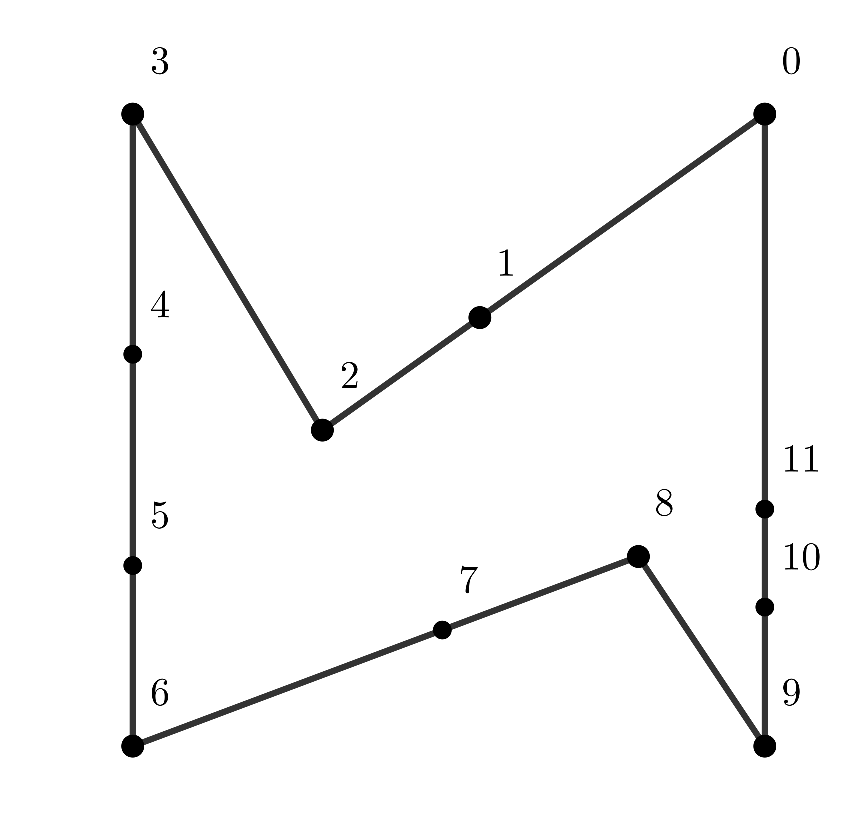
\includegraphics[width=0.9\linewidth]{simple_bit_inserted.eps}
\end{subfigure}%
\begin{subfigure}{0.5\columnwidth}
\centering
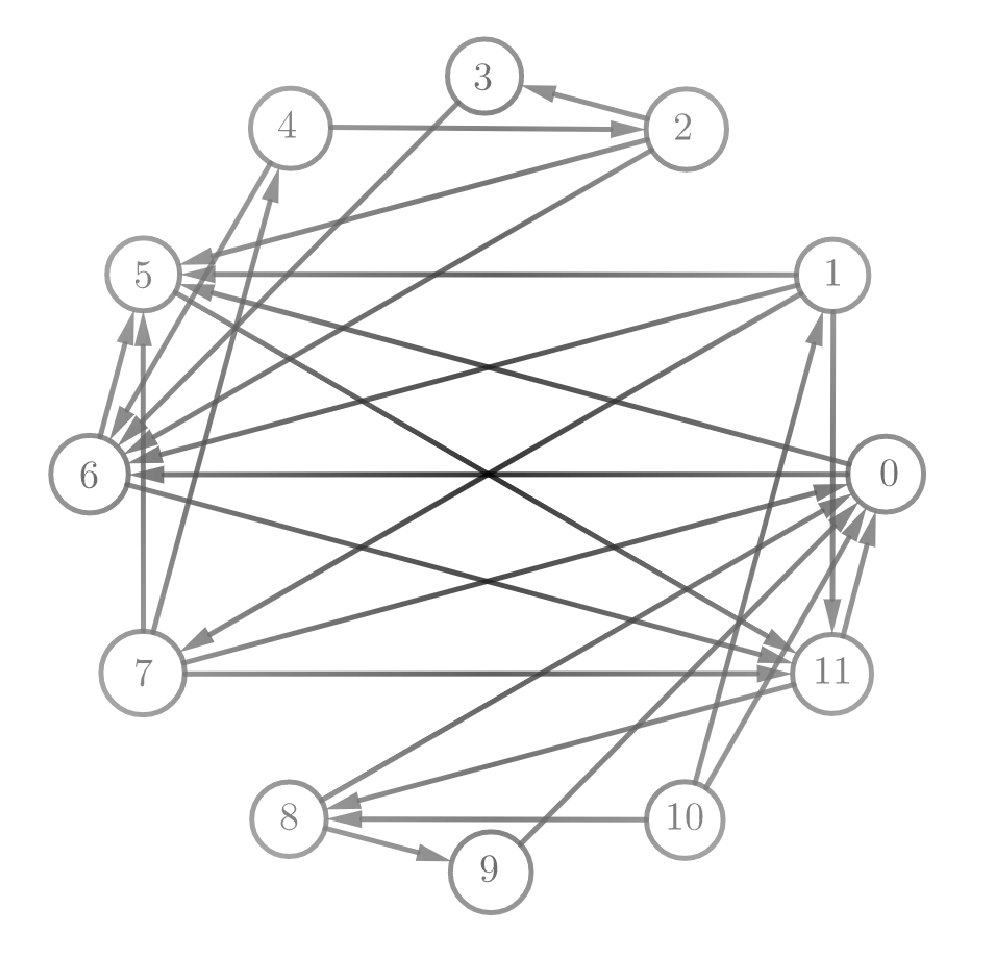
\includegraphics[width=0.9\linewidth]{simple_bit_safe_graph.eps}
\end{subfigure}
\caption{A polygon after Algorithm \ref{algo:insert} and its safe bounce visibility graph $BVG_{safe}$. }
\label{fig:simple_bit}
\end{figure}


\subsubsection{Constant Strategy Search}

Despite a lack of complete reachability, we would like to have a tool to
compute safe nondeterministic 
controllers of minimal complexity, for applications such as micro-scale
robotics. Here, we will show how to
search for a constant fixed-angle bounce controller, where at every stage the
robot executes a fixed-angle bounce in some range $\tilde{\theta}$. This is an
extension of the controllers analyzed in \cite{NilBecLav17} for regular polygons.
We define the functions:

\begin{itemize}
\item \textsc{mkBVG}: Uses the visibility information generated in Algorithm
\ref{algo:insert} to generate the bounce visibility graph in $O(n^4)$ time.
\item \textsc{mkSafeBVG}: Using Definition \ref{def:sa} and Proposition \ref{prop:saferange}, we can create a \emph{safe roadmap}, $G_{safe}$,
        out of the bounce visibility graph by traversing all edges and removing edges with an 
        empty $\tilde{\theta}$, and labelling the remaining edges with the interval 
        of safe actions.
\item \textsc{SearchConstantFixedStrats}: performs breadth-first search from
start to goal, starting with $\tilde{\theta} = (0, \pi)$ and intersecting
$\tilde{\theta}$ with the safe action intervals along each path, terminating
when the path reaches the goal state with nonzero
$\tilde{\theta}$ intervals. Returns the resulting constant controller $\tilde{\theta}$ or that
no such strategy is possible.
\end{itemize}

\begin{algorithm}
\caption{\textsc{SafeConstantFixedNavigate}($P$, $S$, $G$, $k$)}
\label{algo:nav}
\hspace*{\algorithmicindent} \textbf{Input:} A polygon $P$, intervals $S$ and
$G$ in $\partial P$, and an integer bound $k$.\\
\hspace*{\algorithmicindent} \textbf{Output:} A nondeterministic bounce rule,
or \textsc{None} if no strategy can be found.
\begin{algorithmic}[1]
\State $P' \gets$ \Call{PartitionPoly}{$P$}
\State $BVG \gets$ \Call{mkBVG}{$P'$}
\State $BVG_{safe} \gets$ \Call{mkSafeBVG}{$BVG$}
\State $\tilde{\theta} \gets$ \Call{SearchConstantFixedStrats}{$BVG_{safe}$, $S$, $G$, $k$}
\State \textbf{return} $\tilde{\theta}$
\end{algorithmic}
\end{algorithm}

\subsubsection{Examples}

Here we provide an example of strategies that can be generated with different
types of search in the safe bounce graph. We will use an example environment
consisting of two convex ``rooms" connected with a corridor. The corridor does
not have parallel sides, in order to make the problem more geometrically
interesting.

Using the \textsc{SafeConstantFixedNavigate} strategy in the environment shown in Figure
\ref{fig:example_env}, we
can show that you cannot reach either ``room" from the other under a constant
strategy. An example feasible constant strategy was generated from edge $e_5$
to edge $e_4$, with the action interval $\tilde{\theta} = (0.0363, 0.1767)$.
This strategy causes the robot to bounce around the right room, and was
validated by choosing random angles in the
interval $(0.0363, 0.1767)$ as seen in Figure \ref{fig:constant}.



When we search for the path using the fewest number of transitions from a start
point on segment $e_0$ to $e_{16}$, we compute the plan

\begin{center}
\begin{tabular}{ c c c c }
 Stage & Start Edge & Next Edge & $\tilde{\theta}$ \\ 
\hline
1 & 0  & 17 & (0.3217, 0.3419) \\
2 & 17 & 6  & (2.4668, 2.6949) \\
3 & 6  & 16 & (1.0382, 1.3940) \\
\end{tabular}
\end{center}


and we can see in Figure \ref{fig:short} that when a random start state is
chosen in edge $e_0$, and a random action from set $\tilde{\theta}$ is chosen at
each stage, that all trajectories successfully reach the goal.

\begin{figure}
\centering
\begin{subfigure}{0.8\columnwidth}
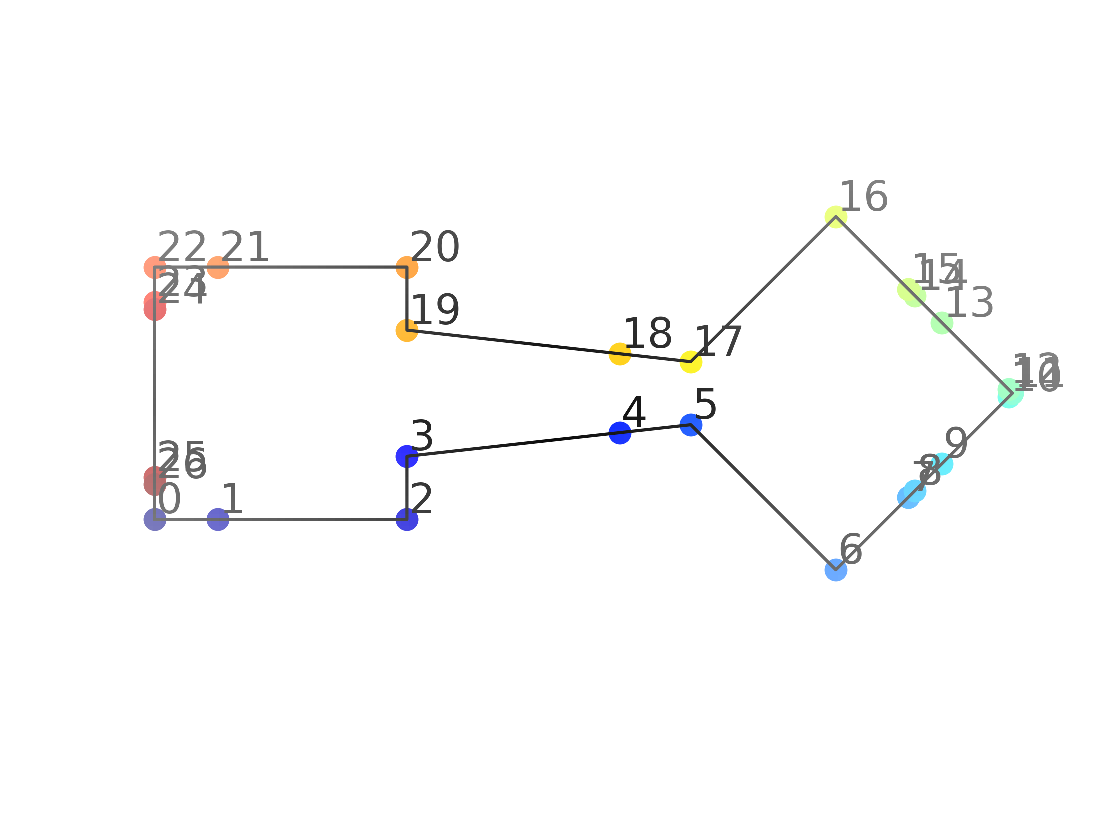
\includegraphics[width=\linewidth]{sort_inserted.eps}
\caption{The example environment, discretized by Algorithm 1. \label{fig:example_env}}
\end{subfigure}
\begin{subfigure}{0.5\columnwidth}
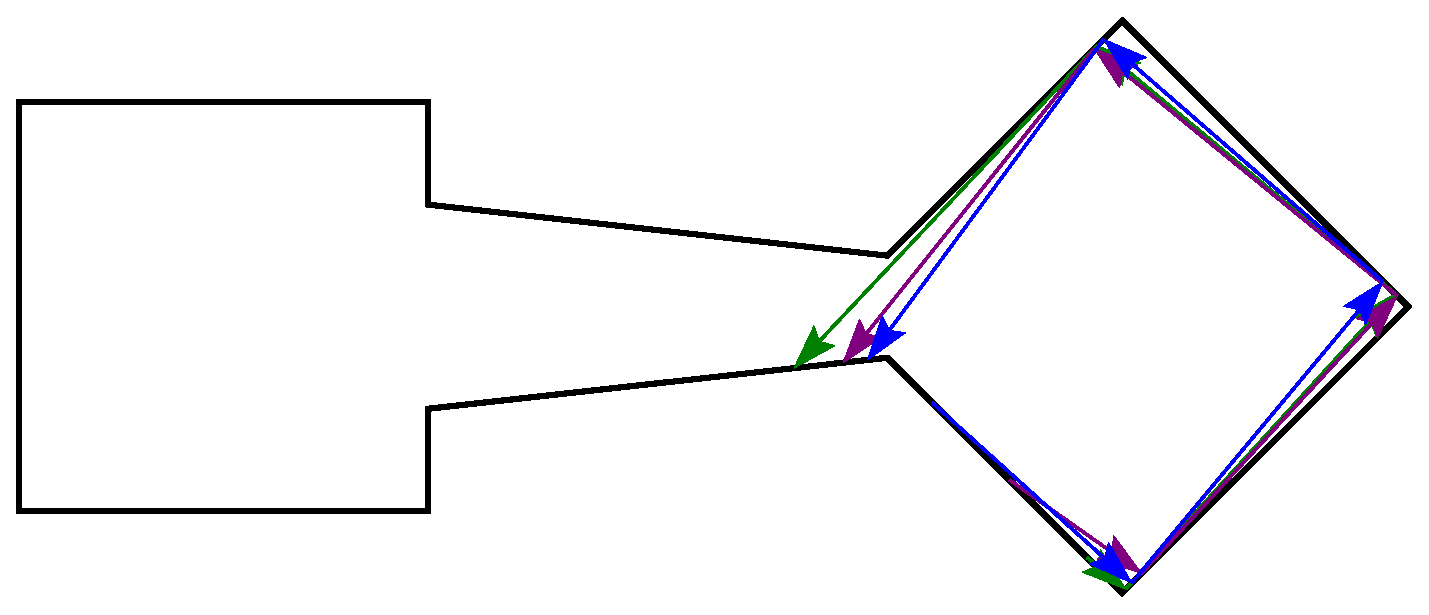
\includegraphics[width=\linewidth]{escape_room.eps}
\caption{A trajectory from edge $e_5$ to edge $e_4$, generated such that the same action set is used at each
stage. \label{fig:constant}}
\end{subfigure}%
\begin{subfigure}{0.5\columnwidth}
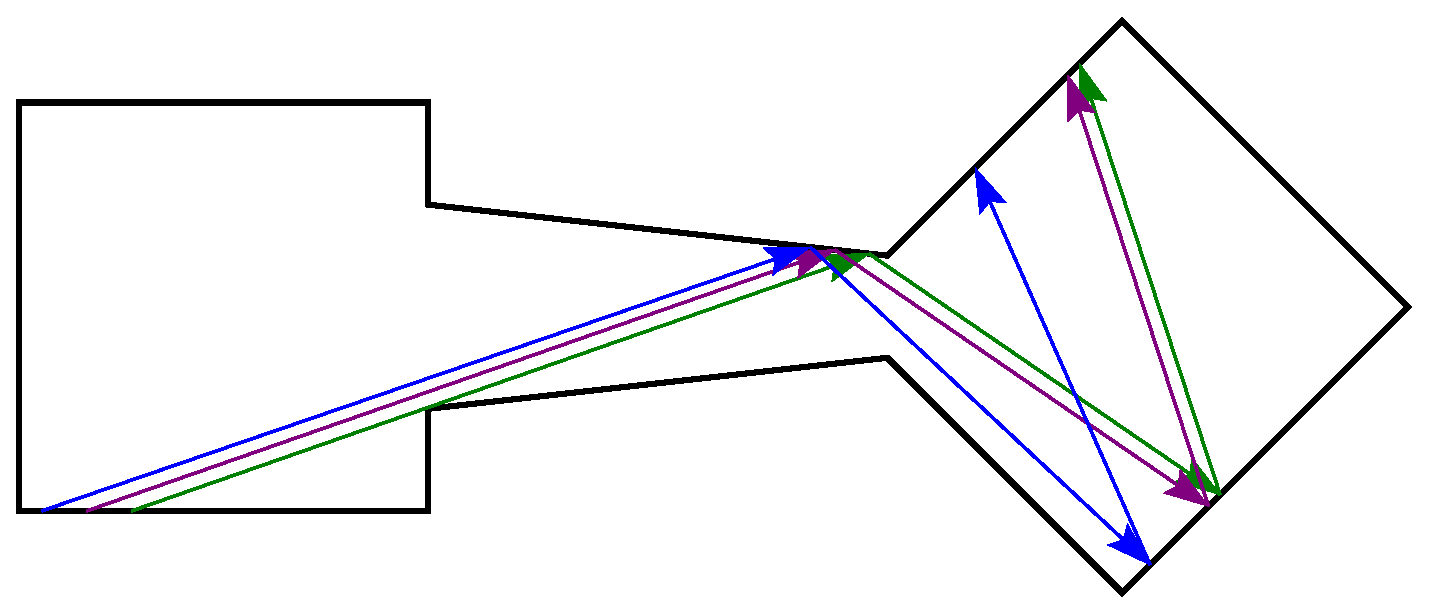
\includegraphics[width=\linewidth]{short_path.eps}
\caption{A trajectory from edge $e_0$ to edge $e_16$ generated with the fewest number of bounces.
\label{fig:short}}
\end{subfigure}
\caption{\label{fig:examples}}
%}
\end{figure}


However, we notice that the action intervals at each stage are quite small,
requiring accuracy from the robot of $0.02$ radians, or about 1.15 degrees. To
address this and improve tolerance for uncertainty, there are several options.
For example, we can set a minimum uncertainty (size of action set) and search for paths until
we find one with at least that size. We may also search for the path (of under a
certain bounded number of transitions) with the largest minimum action set.


\subsection{Patrolling}

In Section \ref{sec:limcycles}, we
detailed results on the existence and structure of convex limit cycles in convex
polygons, as well as how cycles can be used in general to reduce uncertainty in
robot position. However, when considering how to plan trajectories including
cycles, it is important to note that there are
exponentially many possible limit cycles (in the size of the polygon), even
if we restrict our controller to a fixed bounce rule. The
main reason for this is that a cycle may contain
transitions which are not contraction mappings, as long as the overall
contraction coefficient is less than one.

However, it is possible to take any given
sequence of edges in a polygon and check if the sequence admits a
stable limit cycle, by searching over the bounce rules at each stage for rules
that cause an overall contraction coefficient to be less than one and satisfy
the geometric constraints. As more becomes understood about the structure and robustness of
the limit cycles, we can begin to formalize robotic \emph{patrolling} tasks as a search
over possible cycles. Here, we will outline the general form of the patrolling
problem.

\begin{definition}
Given an environment $P$, a set of possible starting states $S$, and
a sequence of edges of the environment $E = \{e_1, \ldots, e_k\}$,
determine a strategy which causes the robot to enter a stable cycle visiting 
each edge of the sequence in order from any point in $S$.
\end{definition}

This task is related to the Aquarium Keeper's Problem in computational
geometry \cite{czyzowicz1991aquarium}. It may be solved by coloring nodes in the
bounce visibility graph by which edge of $P$ they belong to, and then searching
for cycles which visit edges in the correct order. If a cycle is
contracting, it will result in a converging stable trajectory. Interesting open questions 
remain on how to incorporate other useful properties of a
patrolling cycle, such as coverage of a space with certain sensors, or guarantees
about detecting evaders while patrolling. We are also interested in how to use
heuristics and approximate methods to more efficiently search for such cycles, since it
 is equivalent to the travelling saleman problem and is therefore NP-hard.



\begin{figure}
\centering
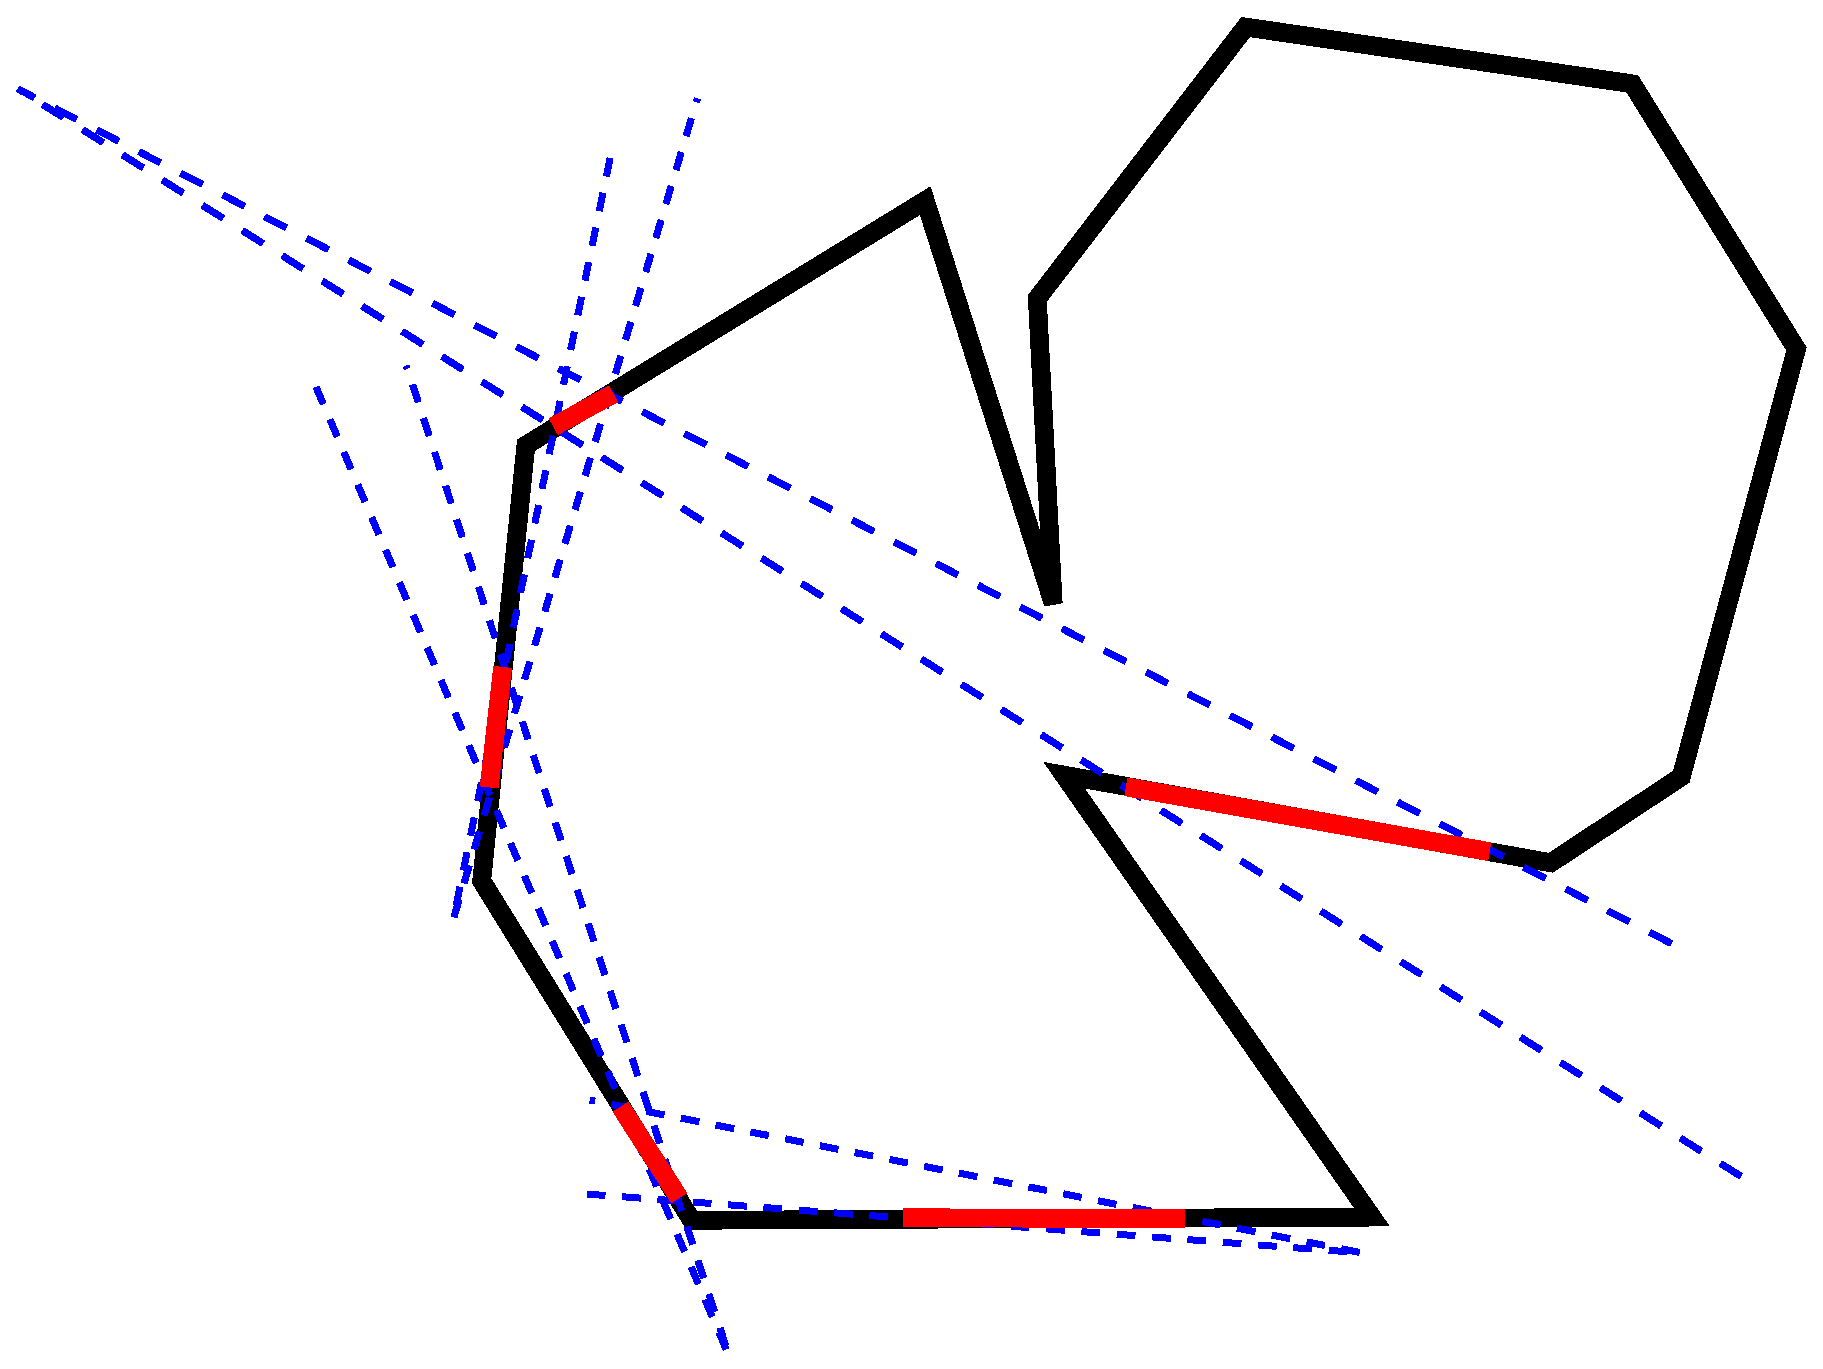
\includegraphics[width=0.8\columnwidth]{bounce_preimages.eps}
\caption{An example of how contraction properties can be used to control
robot state uncertainty enough to navigate the robot through a narrow doorway
with nondeterministic actions.}
\label{fig:preimage_example}
\end{figure}


\section{Open Questions and Future Work}

We have presented a visibility-based approach to reasoning about 
paths and strategies for a class of mobile robots. We are moving toward
understanding nondeterministic control of such robots; however, many open
questions remain!

\textbf{Comparing bounce rules.} Our approach can be used to compare different families of
bounce strategies in a given polygon, by comparing the reachability of the
transition systems induced by each strategy family. This would require 
either reducing the full bounce visibility graph given constraints on
possible bounces, or constructing a more appropriate transition
system. It is not clear the best way to analyze relative bounce rules, in which the
outgoing angle of a robot after a collision is a function of the incoming angle.

\textbf{Optimal Strategies.} Say we wish to
find the strategy taking the robot from region $S$ to region $G$ with the
maximum amount of allowed uncertainty in the bounce rules (the sum of the
interval sizes of each action set along the path). We may also wish find sequences of
transitions which are optimally contracting (maximally reduce uncertainty in robot
position and effect of nondeterminism). These problems can be framed as
an optimization problem over the space of all transition function compositions,
or could be solved with search algorithms such as $A^*$ with an appropriately
discretized state space. Future work will address the best approach to finding
such optimal strategies.

\textbf{Localization.} A localization strategy is a nondeterministic strategy that 
produces paths which reduce uncertainty in the robot's position to below some
desired threshold, from arbitrarily large starting sets. The use of limit cycles
to produce localizing strategies has been explored in \cite{alam2018space}, and
it would be interesting to take a similar approach with our environment
discretization.

\textbf{Ergodic Trajectories.} 
We are interested in strategies that produce ergodic motion, where the robot's
trajectory ``evenly'' covers the state space. Measures
of ergodicity have recently been used in exploration tasks
\cite{miller2016ergodic}. Chaotic dynamical systems have also been used directly
as controllers for mobile robots \cite{nakamura2001chaotic}.

\begin{acks}
This work was supported by NSF grants 1035345 and 1328018, and CONACyT
post-doctoral fellowship 277028.
\end{acks}

\bibliographystyle{SageH}
\bibliography{refs}

\end{document}
